\chapter{提案手法} \label{chap:algorithm}
本章では提案手法を詳しく説明する.
まず,\secref{flow}にて自動生成の大まかな流れを説明し,その後にそれぞれの工程について詳しく述べる.
\secref{input}および\secref{output}にて入出力について説明し,
\secref{device}にて使用するデバイス,
\secref{software}にて使用するソフトウェア,
\secref{3Dmodel}にて使用する3Dモデルについて述べる.
\secref{analysis}にてMIDIデータから音情報への変換方法,
\secref{adapt}にて音情報のモーションへの適用方法を説明する.
そして最後に,\secref{howto}にて実際にシステムを使用する際の,使用方法について言及する.

\section{自動生成の流れ} \label{sec:flow}
\figref{fig:flow}に,音源から吹奏アニメーションを自動生成する流れを示す.\\
\begin{figure}[h]
	\centering
	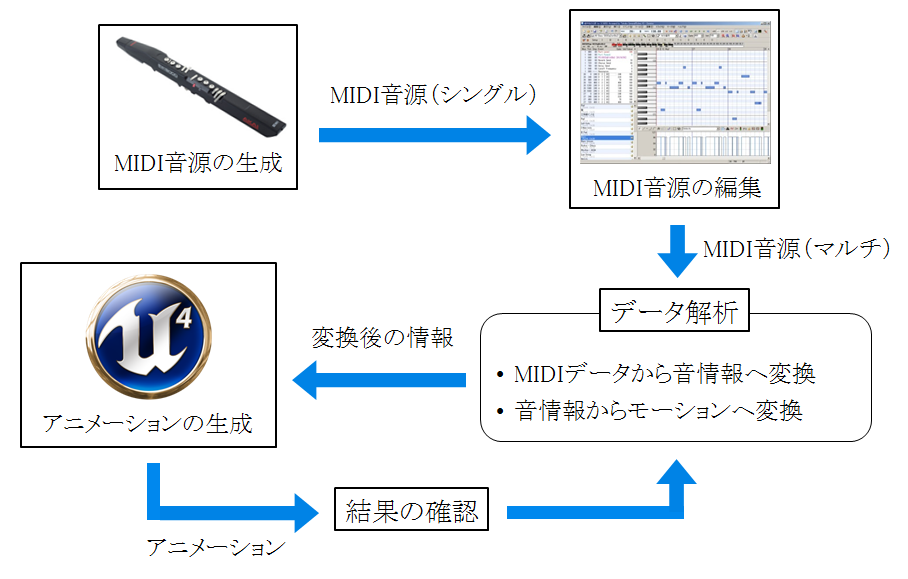
\includegraphics[width=14cm]{fig/chap3/flow.eps}
	\caption{音源から吹奏アニメーションを自動生成する流れ}
	\label{fig:flow}
\end{figure}
\indent
実際のアニメーション制作フローに沿わせるため,音源の生成は楽器を用いて行う.
次に,生成した音源を解析し,譜面データへ変換する.
そして,アニメーション生成と同時に音源を流すことにより,音源に合わせてキャラクタが動くアニメーションが完成となる.

\section{入力} \label{sec:input}
入力する音源は,MIDI音源とする.
ここで,MIDI音源は,MIDIという信号を受信して発音する音源のことである.
よく使用されるmp3やwaveなどの形式とは異なり,中身が譜面データとなっているため,音の解析が比較的容易である.\\
\indent
このMIDI音源を生成する方法は,後述する.

\section{出力} \label{sec:output}
出力は,管楽器を演奏するキャラクタのアニメーションである.
今回対象とする管楽器は,トランペット,トロンボーンである.
この2本の楽器を選んだ理由は,吹奏楽ではとくに目立つ楽器であり,3Dモデルが入手しやすかったために選んだ.

\section{デバイス} \label{sec:device}
MIDI音源を生成するために,電子楽器であるウインドシンセサイザ「EWI5000」(\figref{fig:ewi})を使用する.
このウインドシンセサイザは,さまざまな楽器の音を再現することが可能である.
\begin{figure}[h]
	\centering
	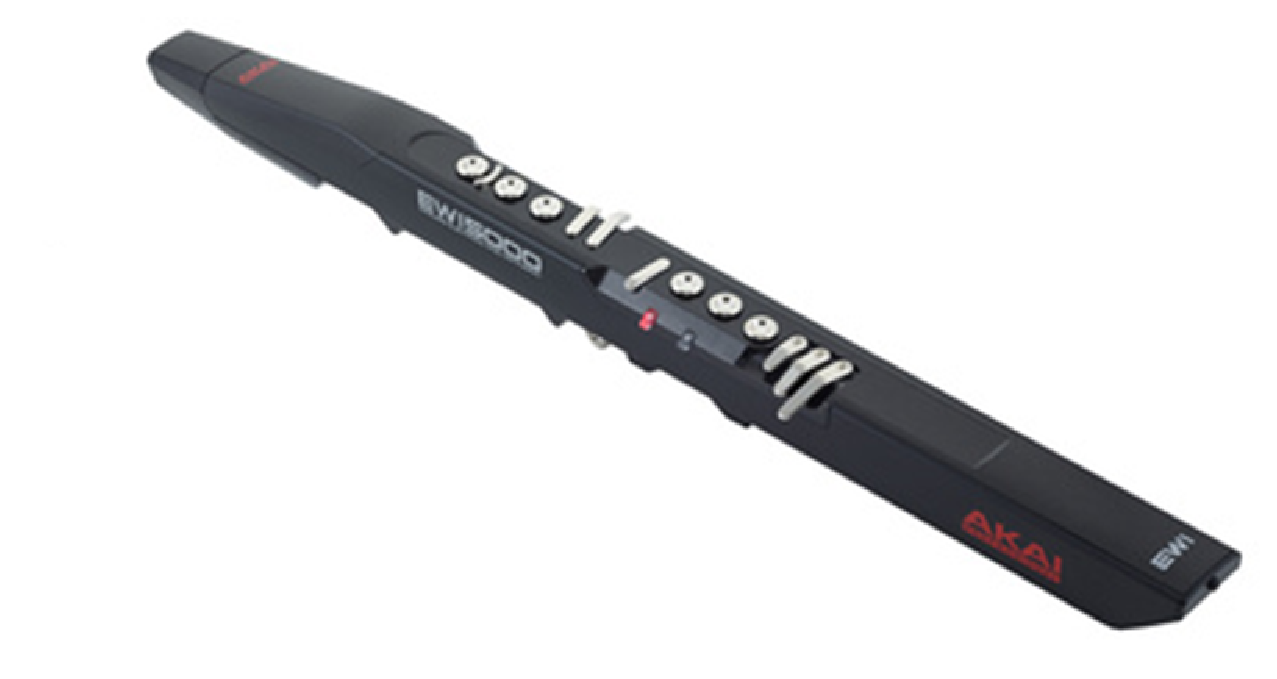
\includegraphics[width=8cm]{fig/chap3/ewi.eps}
	\caption{ウインドシンセサイザ「EWI5000」}
	\label{fig:ewi}
\end{figure}

\section{ソフトウェア} \label{sec:software}
\begin{figure}[h]
	\centering
	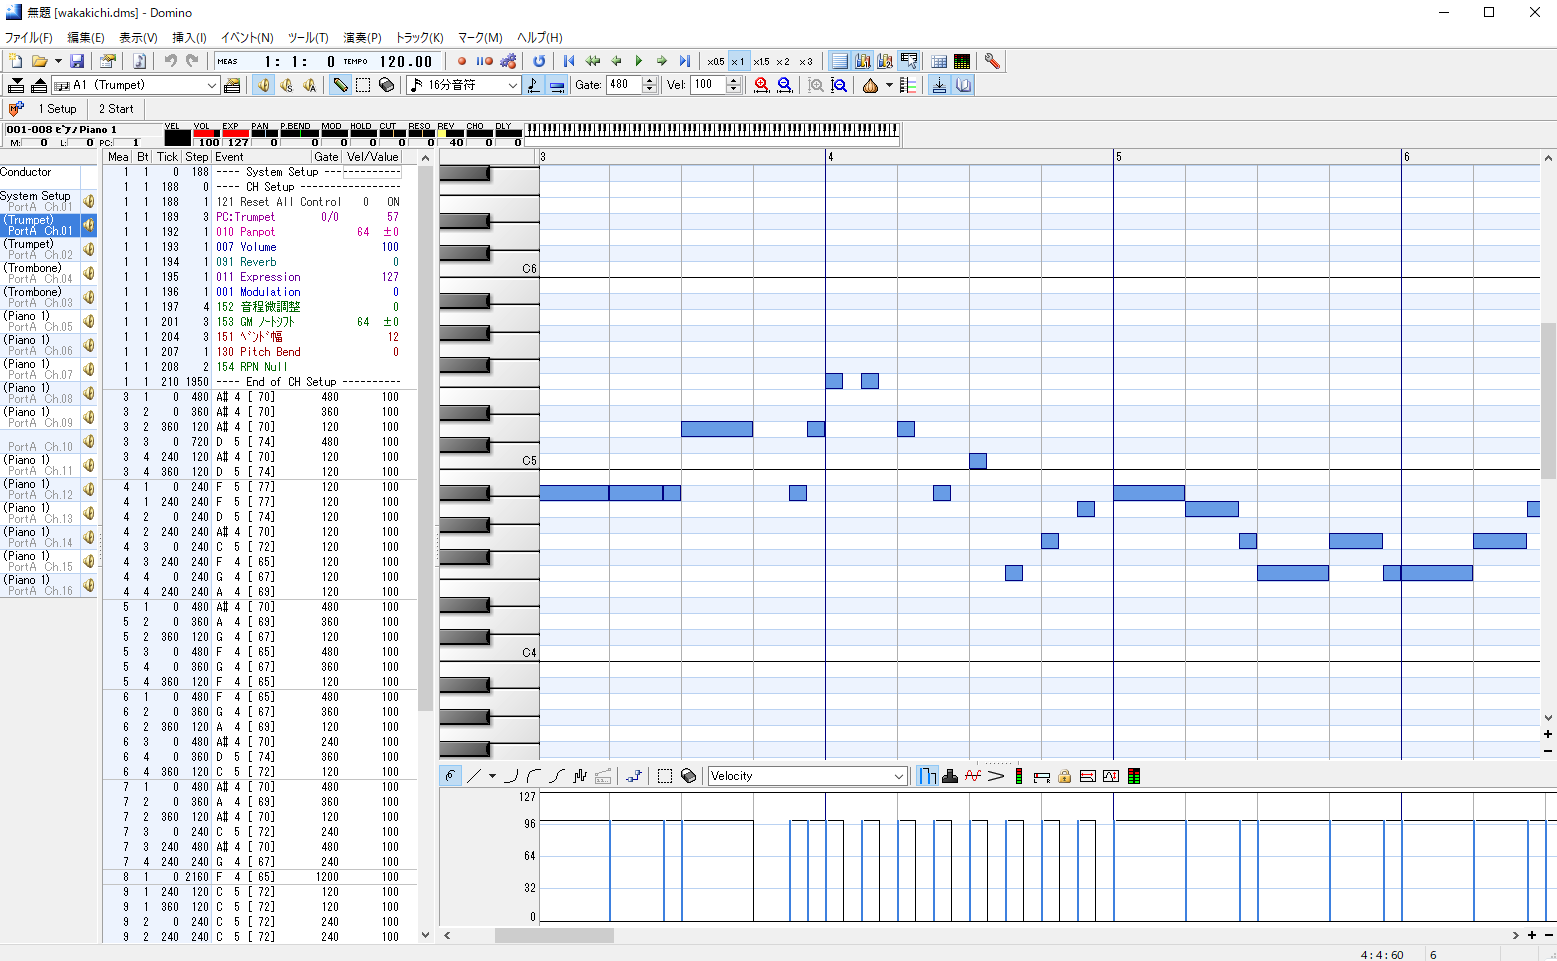
\includegraphics[width=10cm]{fig/chap3/domino.eps}
	\caption{MIDIシーケンスソフトウェア「domino」}
	\label{fig:domino}
\end{figure}
\secref{sec:device}で述べたウインドシンセサイザは,単音しか鳴らすことができないため,シングルチャンネルの音源しか生成することができない.
しかし,吹奏アニメーションを自動生成するためには,複数人で演奏しているマルチチャンネルの音源が必要となる.
そこで,ウインドシンセサイザで生成したMIDI音源を,フリーソフトウェアであるMIDIシーケンスソフトウェア「Domino」(\figref{fig:domino})\cite{domino}に出力し,重ねて何度も録音することにより,マルチチャンネルの音源を生成する.\\
\indent
また,アニメーションの生成には,Epic Gamesより開発されたゲームエンジン,Unreal Engine\cite{ue4}を用いる.

\section{3Dモデル} \label{sec:3Dmodel}
使用する3Dモデルは,
ユニティちゃん(\subfigref{fig:model}{fig:unity}),トランペット(\subfigref{fig:model}{fig:tp}),トロンボーン(\subfigref{fig:model}{fig:tb})である.
\begin{figure}[t]
	\centering
	\subcaptionbox{\textgt{ユニティちゃん}
		\label{fig:unity}}[0.75\linewidth]{
		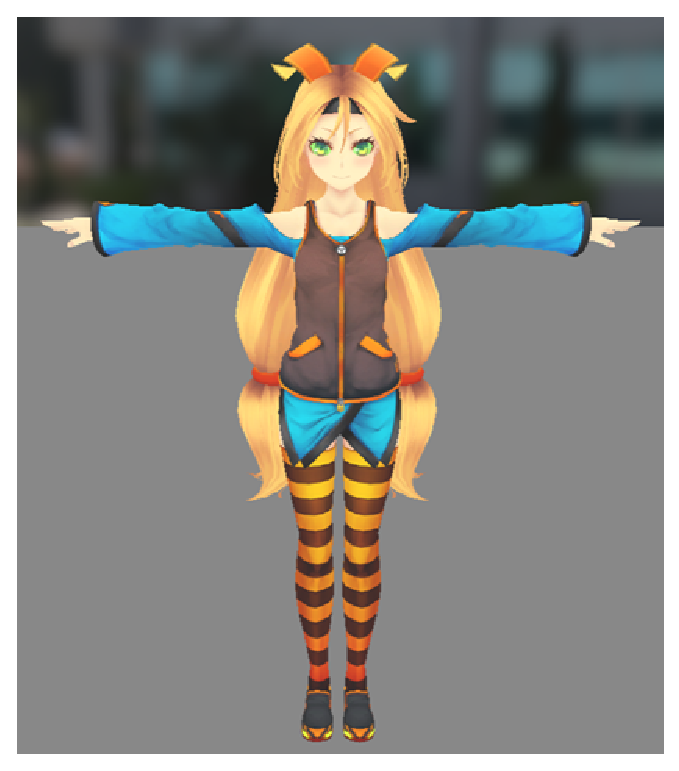
\includegraphics[height=7cm]{fig/chap3/unity.eps}}
	\subcaptionbox{\textgt{トランペット}
		\label{fig:tp}}[0.6\linewidth]{
		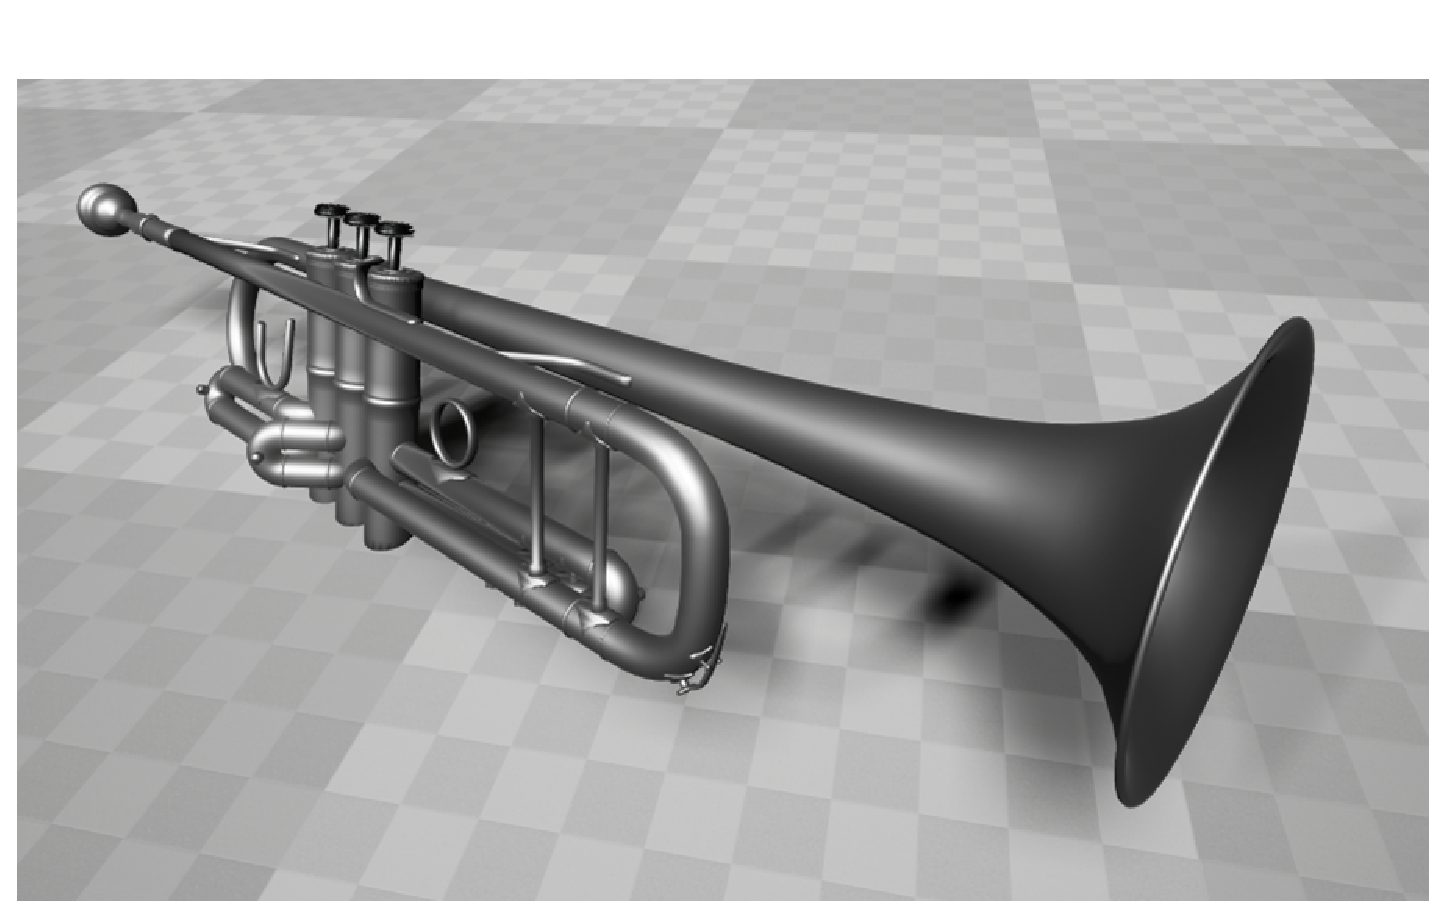
\includegraphics[height=5.5cm]{fig/chap3/tp.eps}}
	\subcaptionbox{\textgt{トロンボーン}
		\label{fig:tb}}[0.6\linewidth]{
		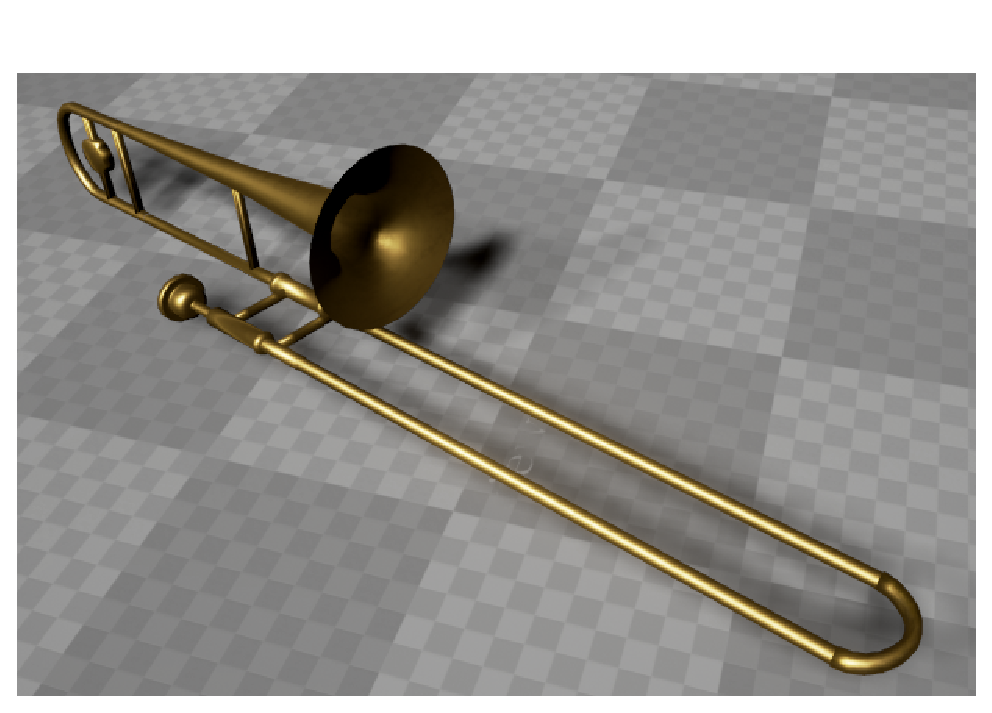
\includegraphics[height=5.5cm]{fig/chap3/tb.eps}}
	\caption{使用する3Dモデル}
	\label{fig:model}
\end{figure}
それぞれ,\cite{unity},\cite{tp},\cite{tb}からダウンロードした.
なお,ユニティちゃんのライセンス条約は,webサイト\cite{license}にて確認済みである.\\
\indent
ユニティちゃんは,主に以下の部位を制御する.
\begin{itemize}
	\item 右指(トランペット演奏時)
	\item 右腕(トロンボーン演奏時)
	\item 背
	\item 腰
	\item 両足
	\item 口元
\end{itemize}
\section{MIDIデータから音情報への変換} \label{sec:analysis}
MIDIは,チャンクとよばれるデータブロックから構成され,先頭にヘッダチャンク,その後にトラックチャンクが続く.
ヘッダチャンクには,チャンクタイプ,データ長さ,フォーマットタイプ,トラック数,タイムベース値という5つの値が格納されている.
ここで,タイムベース値とは,四分音符1つが何クロックになるのかを表す値であり,一般的には48から960までの数字の中の,96の倍数が用いられやすい.
一方トラックチャンクには,チャンクタイプ,データ長,トラックイベントデータが格納されている.
提案手法では,これらの中からトラック数,タイムベース値,トラックイベントデータを楽譜データに変換した後に,アニメーションに適用できる形へとさらに変更する.
\indent
まず,音に関する情報を楽譜データに変換する方法について説明する.
テンポ情報は,四分音符あたり何マイクロ秒なのか,という形で格納されている.
音に関する情報は,トラックイベントデータとして以下のように16進数で格納されている.\\

\hspace{10mm}9 0 4 8 6 4 8 1 7 0 8 0 4 8 0 0 8 3 6 0\\

この情報を以下のように2つずつペアにし,そこから音の種類と長さを取得する.\\

\begin{itemize}
	\item 90: ノートオン.このタイミングで音を鳴らすことを意味する.
	\item 48: 音の種類(48はドを意味する.対応表は次項にて示す.)
	\item 64: 音の大きさ
	\item 81: 音を鳴らしている長さ(前半)
	\item 70: 音を鳴らしている長さ(後半)
	\item 90: ノートオフ.このタイミングで音を止めることを意味する.
	\item 48: 音の種類(48はドを意味する.)
	\item 00: 音の大きさ(音を止めているため,大きさはゼロとなる.)
	\item 83: 音を止めている長さ(前半)
	\item 60: 音を止めている長さ(後半)
\end{itemize}

音の長さは,以下のように10進数に変換する.ここでは,81 70を用いて説明する.\\

\begin{itemize}
	\item まず,それぞれを2進数に変換する.\hspace{1mm}81: 1000 0001,70: 0111 0000
	\item そして,それぞれの最上位ビットを取り除いて合成し,10進数に直す.\hspace{1mm}000 0001 111 0000 → 240
\end{itemize}

この例の場合,ドを240クロック分伸ばすことを意味する.以降,この値をデルタタイムとよぶ.\\
\indent
デルタタイムを楽譜の情報に直すには,\secref{sec:analysis}の冒頭で述べたタイムベース値を用いる.


最後に,このクロックを現実時間[s]に変換する.変換式は,\eqref{eq:eq1}で表される.
\begin{equation}
\label{eq:eq1}
時間[s] = 
\frac {デルタタイム[ticks] × 60[seconds/minute]}{タイムベース値[ticks/beat] * テンポ[beats/minute]}
\end{equation}

タイムベース値,テンポをそれぞれ仮に480,120とすると,例で示した音情報は,譜面情報に直した結果『ドを0.25秒伸ばし,0.5秒休む』ことを意味すると分かる.

\section{音情報のモーションへの適用} \label{adapt}
\subsection{指や腕,楽器のパーツへの適用}
音を鳴らしている様子をアニメーションで再現するには,キャラクタの指や腕を介して楽器を制御する必要がある.
トランペットはピストンの操作,トロンボーンはスライド管の操作により音を変えることができ,ピストンは3箇所,スライド管は止める場所が大きく分けて7箇所ある.
トランペットのピストン番号を,吹き口に近い方から1-3(\subfigref{fig:numbering}{fig:piston}),トロンボーンのスライドの位置を,吹き口に近い方から1-7(\subfigref{fig:numbering}{fig:slide})と表すと,MIDIデータと音,運指の対応は\tabref{tab:map}となる.

\begin{figure}[t]
	\centering
	\subcaptionbox{\textgt{ピストン番号}
		\label{fig:piston}}{
		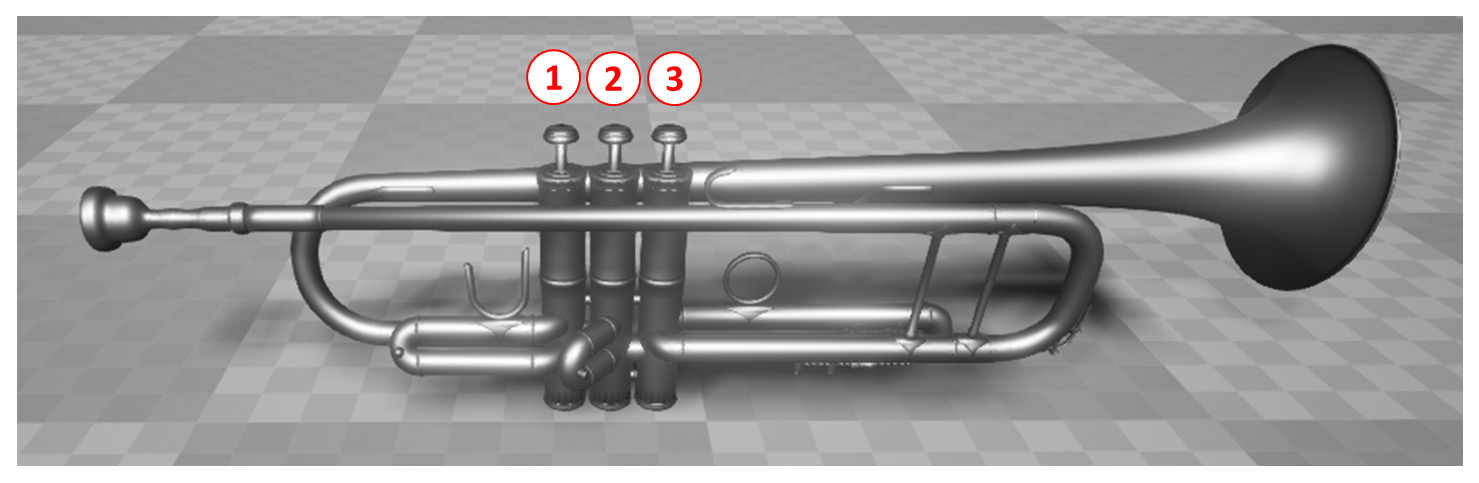
\includegraphics[height=3cm]{fig/chap3/tp_piston.eps}}
	\subcaptionbox{\textgt{スライドの位置番号}
		\label{fig:slide}}{
		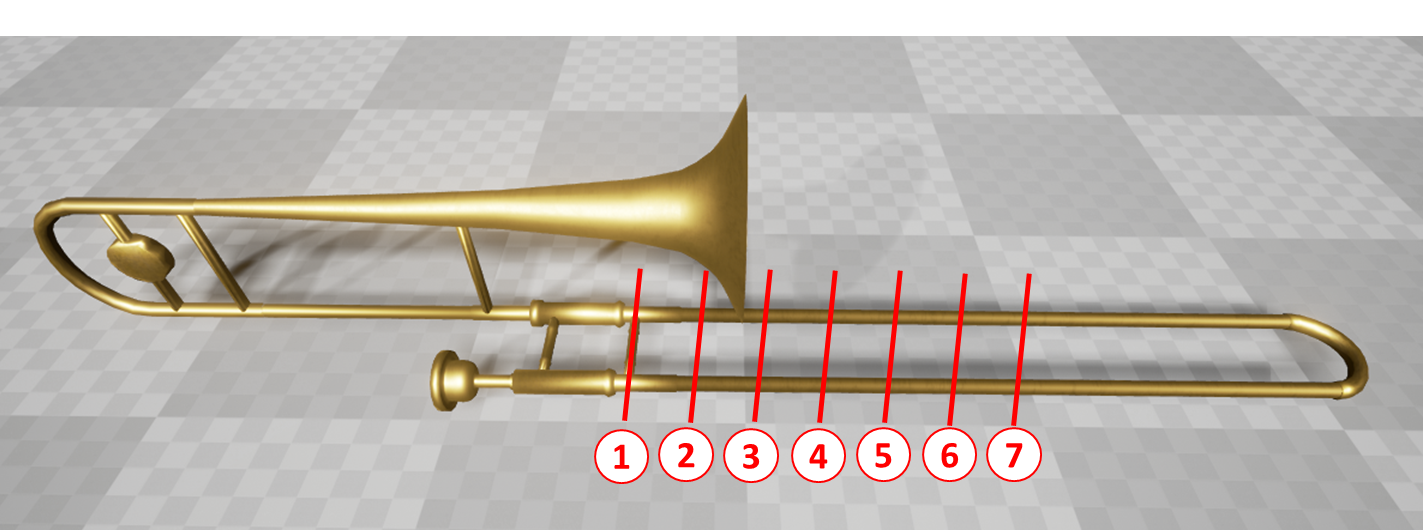
\includegraphics[height=5cm]{fig/chap3/tb_slide.eps}}
	\caption{番号付け}
	\label{fig:numbering}
\end{figure}

\begin{table}[h]
	\centering
	\caption{MIDIデータと音,運指の対応}
	\begin{tabular}{|c|c|c|c|} \hline
		MIDIデータ & 音名(実音) & トランペット & トロンボーン \\ \hline \hline
		\vdots & \vdots & \vdots & \vdots \\ \hline
		39 & A(ラ,442Hz) & 2 & 2 \\ \hline
		3b & B(シ) & 1・2・3 & 4 \\ \hline
		3c & C(ド) & 1・3 & 3 \\ \hline
		3e & D(レ) & 1・2 & 1 \\ \hline
		40 & E(ミ) & 2 & 2 \\ \hline
		41 & F(ファ) & 0 & 1 \\ \hline
		43 & G(ソ) & 1・2 & 2 \\ \hline
		45 & A(ラ) & 2 & 2 \\ \hline
		\vdots & \vdots & \vdots & \vdots \\ \hline
	\end{tabular}
	\label{tab:map}
\end{table}

\secref{}で例として挙げた,『ドを0.25秒伸ばし,0.5秒休む』という譜形を演奏する場合,トランペットの場合は,1番と3番を0.25秒間押し続け,その後0.5秒間は休みのためそのまま,トロンボーンの場合は,スライドを3番まで移動させ,そのまま0.25秒間維持,その後0.5秒間は休みのためそのまま,という表現方法となる.\\

\subsection{口元のメッシュへの適用}
\indent
金管楽器を演奏する際,高音域の演奏時は,低音域に比べて口元が緊張する.
緊張の程度には個人差があるが,本論文では,高音演奏時と低音演奏時の口元の違いを\subfigref{fig:mouth}のように,口の引き具合で表す.\\
\begin{figure}[t]
	\centering
	\subcaptionbox{\textgt{低音域演奏時}
		\label{fig:low}}[0.45\linewidth]{
		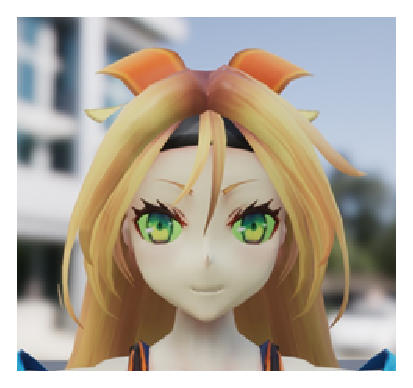
\includegraphics[height=5cm]{fig/chap3/low.eps}}
	\subcaptionbox{\textgt{高音域演奏時}
		\label{fig:high}}[0.45\linewidth]{
		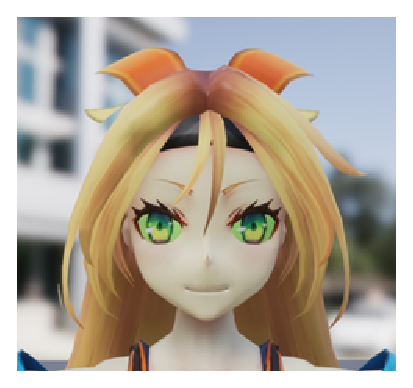
\includegraphics[height=5cm]{fig/chap3/high.eps}}
	\caption{音域による口元の変化}
	\label{fig:mouth}
\end{figure}
\indent
休みが一定の時間以上続く場合,演奏者は息継ぎを行う.息継ぎのタイミングには個人差があり,演奏しているフレーズによっても異なるが,提案手法では息継ぎのタイミングを以下の3パターンに分ける.\\
\begin{itemize}
	\item 休みが0.5拍以上~1拍未満: 休みの間,ずっと息継ぎのモーションを行う.
	\item 休みが1拍以上~2拍未満: 最後の1拍で息継ぎのモーションを行う.
	\item 休みが2拍以上: 最後の2拍間で,息継ぎの予備モーションおよび息継ぎのモーションを行う.
\end{itemize}

息継ぎのモーションを行うときに,口元を\figref{fig:breath}のように変形させる.

口元の制御について
発表の場で申した通り,表情は口元のみ制御していますが,そのためには,メッシュを制御する必要があります.
Unreal Engineでメッシュを制御する際,モーフターゲットという機能を用いますが,この機能はブレンドシェイプが適用されていないメッシュには使用できません.
ここで,ブレンドシェイプとは,あらかじめ用意された複数の表情モデルをパラメタの調整により組み合わせることで,さまざまな表情を作成するアニメーション手法をさします.


その他のモーションについては次項で述べる.\\
\begin{figure}[h]
	\centering
	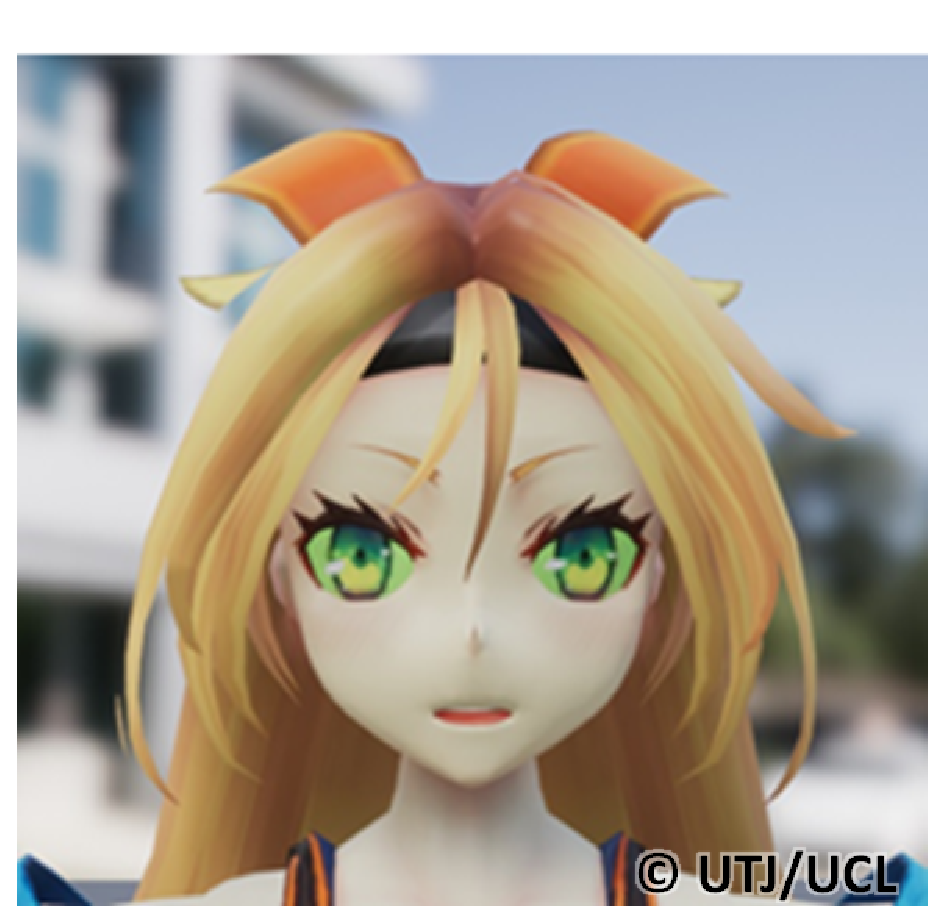
\includegraphics[width=5cm]{fig/chap3/breath.eps}
	\caption{息継ぎをするときの口元}
	\label{fig:breath}
\end{figure}

\subsection{その他の部位への適用}
\indent
息継ぎをするときは口元だけでなく,上半身も動く.
そこで,前項で述べたタイミングで,息継ぎのモーション\subfigref{fig:breath}{fig:up},息継ぎの予備モーション\subfigref{fig:breath}{fig:down}を行う.
なお,比較対象として通常の直立状態を\subfigref{fig:breath}{fig:default}に示すが,差が分かりづらい場合は,楽器と床の端の位置関係を見てほしい.\\
\begin{figure}[t]
	\centering
	\subcaptionbox{\textgt{通常の直立状態}
		\label{fig:default}}[0.45\linewidth]{
		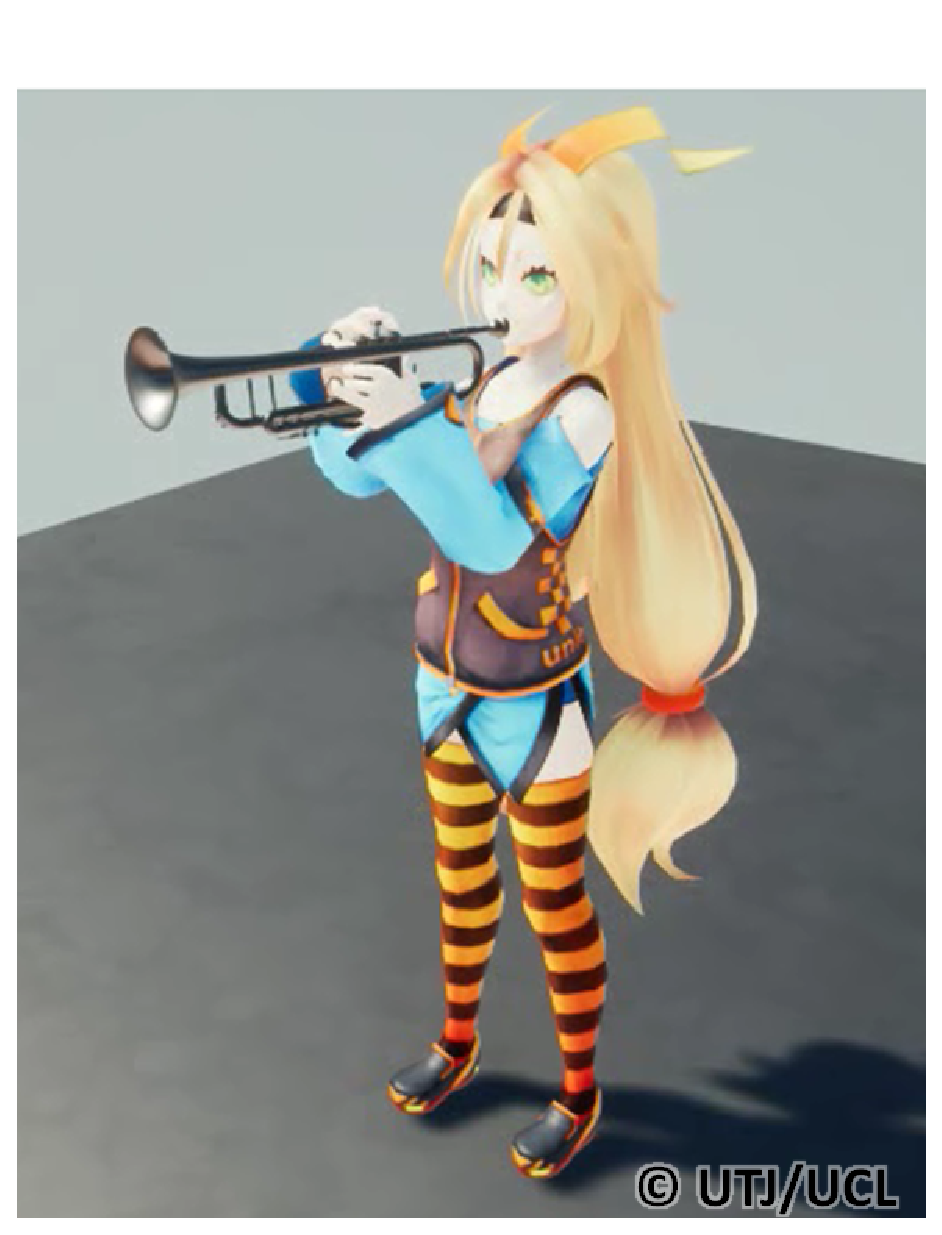
\includegraphics[height=7cm]{fig/chap3/default.eps}}
	\subcaptionbox{\textgt{息継ぎのモーションの最中}
		\label{fig:up}}[0.45\linewidth]{
		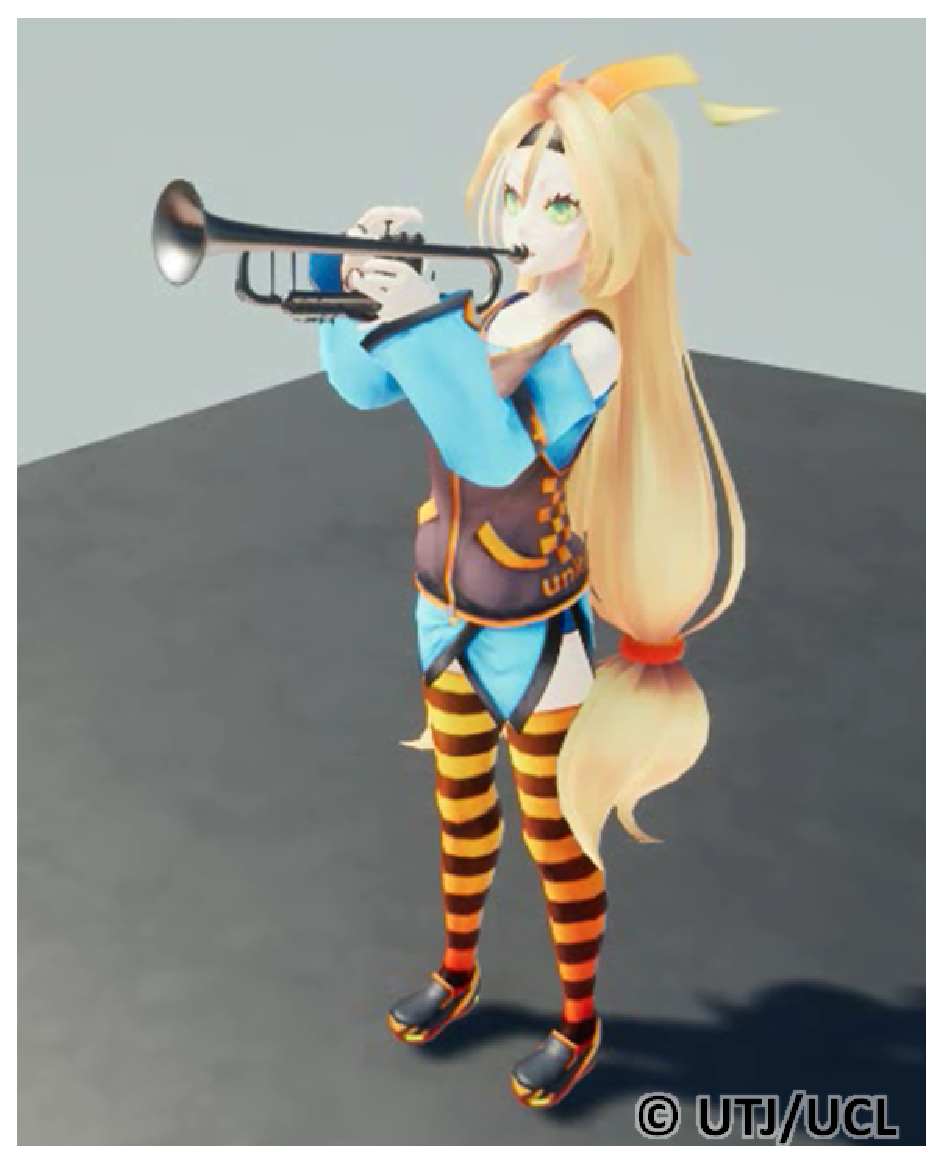
\includegraphics[height=7cm]{fig/chap3/up.eps}}
	\subcaptionbox{\textgt{息継ぎの予備モーションの最中}
		\label{fig:down}}[0.45\linewidth]{
		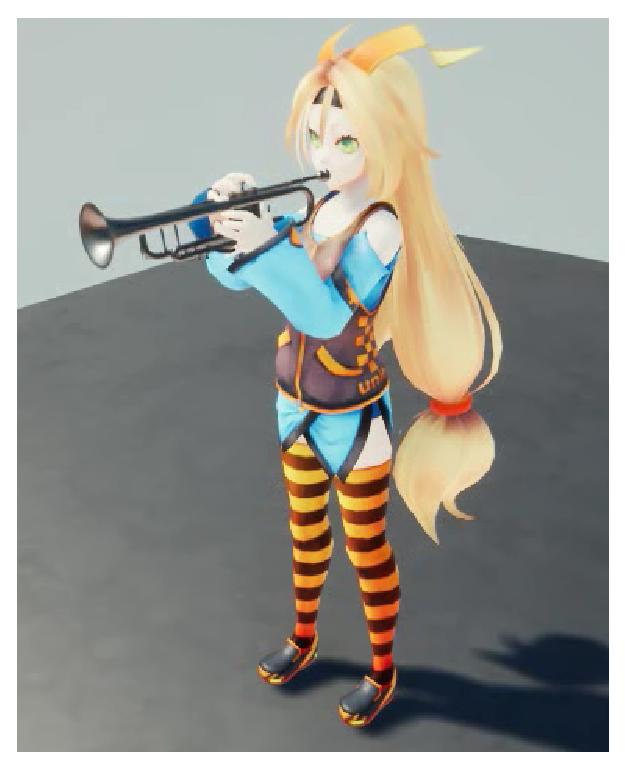
\includegraphics[height=7cm]{fig/chap3/down.eps}}
	\caption{息継ぎ時のモーション}
	\label{fig:breath}
\end{figure}
\indent
息継ぎ時以外にも演奏者は動く.
例えば,任意のタイミングで重心を移動したり,テンポに合わせて身体や楽器を上下に揺らす.
複数人で演奏する際は,基となる1つのモーションのパラメタをランダムに変更することにより,全員に異なる動きを適用する.
また,曲の始まりと終わりを全員で合わせるため,楽器や身体で合図を行う.
これらのモーションは,同研究室学士4年の武内が担当した.
%音情報から一意に定義可能なモーションは堀井.\\

\section{提案手法の使用方法} \label{sec:howto}
提案手法を用いてアニメーションを自動生成する際は,以下の順序が必要となる.
ここで,キャラクタや楽器のモデルは,あらかじめセッティングされているものとする.
\begin{enumerate}
	\item MIDI音源の作成
	\item 音源データの相対パスをコードに記載し,コンパイル
	\item Unreal Engine 4を起動
	\item 1.で生成した音源をBGMとして設定
	\item 再生
	\item 結果の確認および修正
\end{enumerate}\par
手順4.について,本来ならMIDI音源を解析すると同時に音を流すべきであるが,現在の実装ではそれが不可能となっているため,解析する音源とは別に,流す音源として新たに設定する必要がある.
また,このとき音のずれが生じる場合がある.その場合は少しの修正が必要となるが,最初の音だけを合わせることにより,それ以降はアニメーションと音が完全に一致する.